
\section{Soil water content}

\subsection{Definition}
Soil water or moisture content is a ratio, which ranges from 0, meaning completely dry, to the value of material porosity at saturation. It expresses the quantity of water contained in the soil. We can measure it by mass (gravimetric method) or by volume, as depicted in Figure \ref{fig:soil-phase-diagram}. 

We can express this mathematically for volumetric content as
\begin{equation}
    \label{equation:volumetric-content} \theta = \dfrac{V_w}{V_s + V_w + V_a}
\end{equation}
where $V_w$ is the volume of water and $V_s + V_w + V_a$ is the total volume of the soil sample including contained air. Likewise, gravimetric water content is defined as
\begin{equation}
    \label{equation:gravimetric-content} u = \dfrac{m_w}{m_s}
\end{equation}
where $m_w$ is the mass of the water and $m_s$ is mass of all solids in the sample.

\begin{figure}
    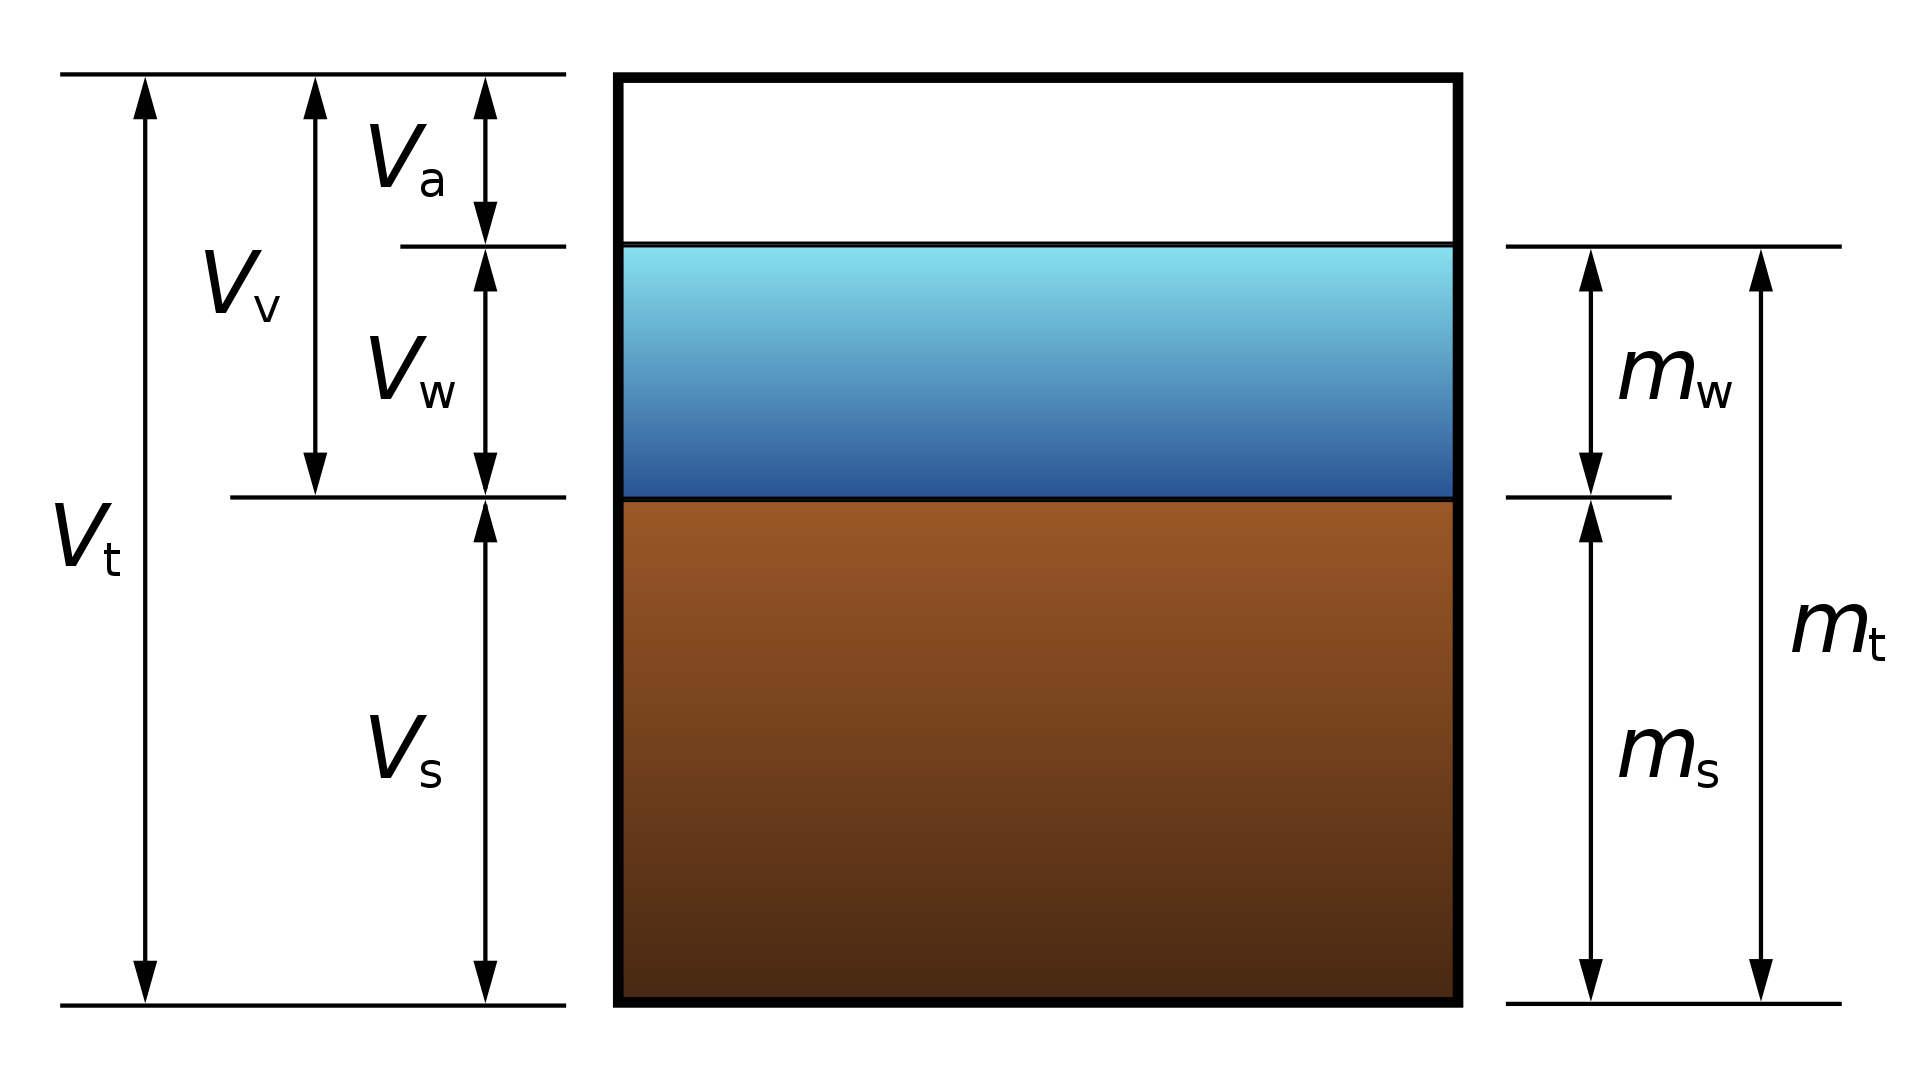
\includegraphics[width=.8\textwidth]{fig/soil-phase-diagram.png}
    \caption{\label{fig:soil-phase-diagram} Soil composition by volume and mass}
    %https://en.wikipedia.org/wiki/Water_content#/media/File:Soil-phase-diagram.svg
\end{figure}

\subsection{Methods of measurement}
\subsubsection{Drying the soil}
Drying the soil sample in a drying oven is a direct method of measurement and is used as the reference method. By weighing the sample and also measuring its volume, then doing that again after drying, it is possible to very accurately measure both the volumetric and the gravimetric water content both at the same time.

rozepsat konkretni hodnoty (teplota, cas), je to ve webster. Mozna pridat fotku pred a po pro ilustraci?

Since direct methods of measurement of soil moisture content are impractical for field use, we will focus on indirect methods next.

\subsubsection{Geophysical methods}

\subsubsection{Satellite remote sensing method}
Thanks to recent and ongoing large-scale deployments of Synthetic Aperture Radar satellites, it is possible, that for global-scale soil water content estimation this method will become much more wide-spread. It also relies on the large contrast in dielectric properties of wet and dry soil.

mozna pridat nejakou mapku pro ilustraci?
